\documentclass{article}

\usepackage{ragged2e}
\usepackage{graphicx}
\usepackage{amsmath}
\usepackage{siunitx}

\begin{document}

\begin{flushright}
    \noindent
    Rodrigo Becerril Ferreyra\\
    CECS 311 Section 01\\
    Lab 1B\\
    2020-01-28 to 2020-02-04
\end{flushright}

\section{Introduction} In this lab, we were tasked with simulating
using a rectifying diode with DC and AC voltage sources in
the program LTspiceVI. DC voltage sources are straightforward,
but AC voltage
sources create a sine wave signal, meaning that they
go up to a certain voltage and go down to the opposite voltage.
This reverse polarity may be undesired for some devices, so
it may be necessary to remove the negative portion of this
sine wave. This is what a rectifying diode is meant to do.

For this lab, we modeled the diode 1N4001, which is made of
silicon and has a typical forward voltage of \(V_f = \SI{0.7}{V}\).

\section{DC Sources} \subsection{Forward Biased}
The first circuit
that we tested was a DC voltage source set at \SI{5}{V}
with a 1N4001 diode and a \SI{1}{k\ohm} resistor connected
in series. The circuit looks like this:

\begin{figure}[h]
    \centering
    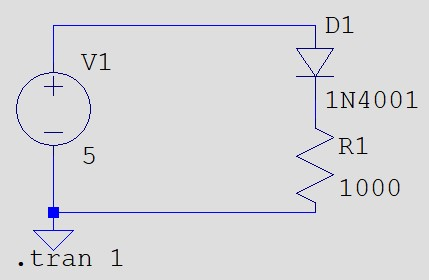
\includegraphics[height=15em]{Images/Circuit1.jpg}
    \caption{Forward Biased DC Circuit}
\end{figure}

This circuit is simple to analyze, because there are no
moving parts. The voltage across the diode should be
the same as its forward voltage, or \(V_D = \SI{0.7}{V}\).
Due to KVL, the resistance across the resistor must be
\(V_R = \SI{5}{V} - \SI{0.7}{V} = \SI{4.3}{V}\).

The output from the simulation is listed below.

\begin{figure}[h]
    \centering
    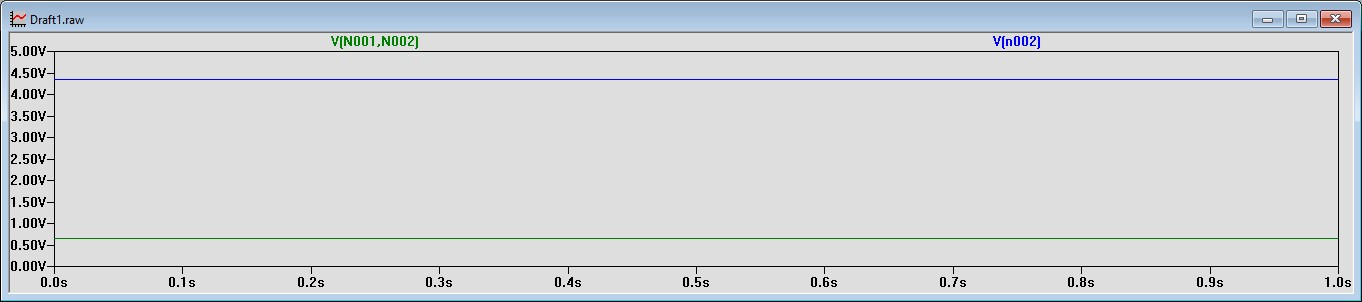
\includegraphics[width=\textwidth]{Images/5VForward.jpg}
    \caption{Graph of output}    
\end{figure}

It may not be very visible on Figure 2, but \(V_D\) drops
just a tiny bit (about \SI{1}{\micro V}) during the first
\SI{0.25}{s}, but is otherwise constant at a measured
\SI{648.737}{mV}, or \SI{0.7}{V}, just as calculated.
\(V_R\) also rises by about \SI{1}{\micro V} during the first
quarter second of the simulation, but is otherwise constantly
\SI{4.35126}{V}, which is close to the expected
\SI{4.3}{V}.

\subsection{Reversed Biased} The next circuit is identical
to the last one minus the fact that the polarity of the
diode has been switched: %insert Circuit2.jpg here

\begin{figure}[h]
    \centering
    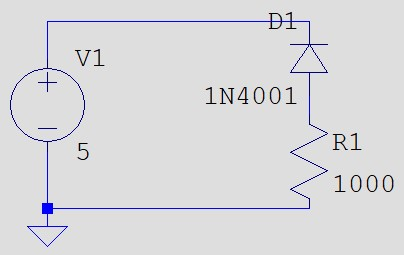
\includegraphics[height=15em]{Images/Circuit1Reverse.jpg}
    \caption{Reversed Biased DC Circuit}
\end{figure}

Because this diode is reverse biased, there is no current going
through the circuit, and therefore by Ohm's Law there is no
voltage drop across the resistor (\(V_R = \SI{0}{V}\)).
This means that the diode is dropping all \(\SI{5}{V} = V_D\).

The output from the simulation of this circuit is shown below. As
it is evident, this is exactly the result found when
measuring the circuit.

\begin{figure}[h]
    \centering
    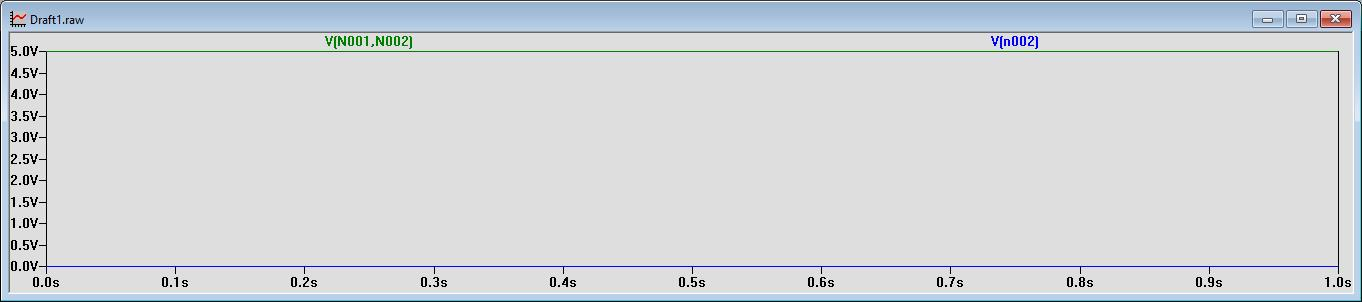
\includegraphics[width=\textwidth]{Images/5VReverse.jpg}
    \caption{Graph of output}
\end{figure}

\section{AC Circuits} When dealing
with a diode and a resistor in series in an AC circuit,
it matters whether you take the voltage across the resistor
or the diode as \(V_\text{out}\), because they behave
differently.
\subsection{Forward Biased} Note that ``forward biased''
is in reference to ground, which in this case is always placed
on the bottom of the voltage source.
The circuit
we are testing is the following:

\begin{figure}[h]
    \centering
    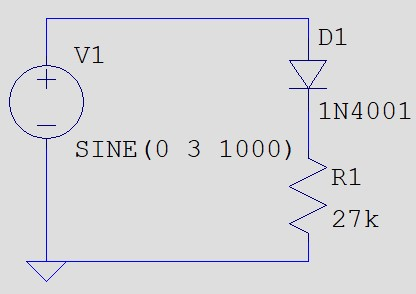
\includegraphics[height=15em]{Images/Circuit2.jpg}
    \caption{Forward biased diode in AC circuit}
\end{figure}

\subsubsection{\(V_\text{out}\) across resistor} 
If \(V_\text{out}\) is taken to be the voltage across the resistor,
this is called a series diode clipper, because it has a diode
in series with the resistor, and it is said to ``clip'' the
negative alternation of the sine wave that the VAC
source outputs. It follows the following function:

\begin{equation}
    V_\text{out}=
    \begin{cases}
        V_\text{in} - V_f & \text{if $V_\text{in} > V_f$}\\
        0 & \text{if $V_\text{in}\le V_f$}
    \end{cases}
\end{equation} Note that in this lab, \(V_\text{in} = \SI3{V} \cdot \sin(x)\)
and \(V_f = \SI{0.7}{V}\).
\(V_\text{out}\) is zero until \(V_\text{in}\) hits \(V_f\),
and therefore will always be
\SI{0.7}{V} below \(V_\text{in}\). \(V_\text{out}\) will never
be negative because a diode does not allow current
to go through it if it is reverse biased.
%What is VAC in pk-pk voltage? What is VR in pk-pk voltage? What is VD in pk-pk voltage?

\subsubsection{\(V_\text{out}\) across diode} If \(V_\text{out}\)
is taken to be the voltage across the diode instead of the
resistor, it is considered to be a shunt diode clipper. The
voltage output therefore follows the following function:
\begin{equation}
    V_\text{out} = 
    \begin{cases}
        V_\text{in} & \text{if $V_\text{in} < V_f$}\\
        V_f         & \text{if $V_\text{in} \ge V_f$}
    \end{cases}
\end{equation} This means that the output voltage will follow
the input voltage until the forward voltage of the diode is
reached: in that case, it will only output that voltage.
For example, for the whole negative alternation and the
beginning and end of the positive alternation
(up to \SI{0.7}{V}), \(V_\text{out}\) will equal \(V_\text{in}\).
However, when \(V_\text{in}\) hits \SI{0.7}{V} and above,
\(V_\text{out}\) will be equal to a constant \SI{0.7}{V}.

\subsubsection{Results} Here is the graph output of both
the series diode clipper and the shunt diode clipper.
The sine wave is \(V_\text{in}\)
(labeled \texttt{V[n001]} or Trace 3), or the output of the
AC voltage source. The line that extends into the negative
region (labeled as \texttt{V[N001, N002]}, or Trace 1)
is the shunt diode clipper, and the line that does
not (labeled as \texttt{V[n002]}, or Trace 2)
is the series diode clipper.

\begin{figure}[h]
    \centering
    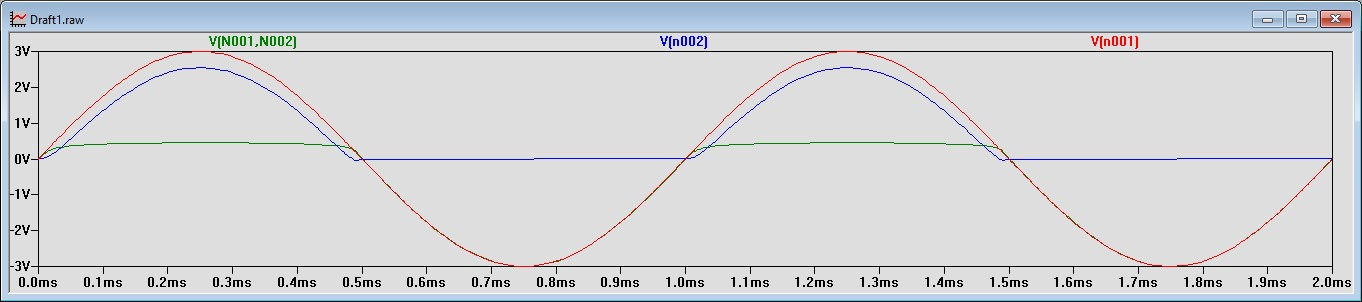
\includegraphics[width=\textwidth]{Images/3VACForward.jpg}
    \caption{Output for both circuits}
\end{figure}

As it is evident, the graph of the output matches the
description. Trace 2 stays under \(V_\text{in}\) and completely
clips off the negative alternation of the sine wave, while
Trace 1 only goes up to \SI{0.7}{V} and follows \(V_\text{in}\)
for its negative alternation.
\(V_\text{in}\) is \(\SI{6}{V}_{pp}\). \(V_{\text{out},R}\)
is \(\SI{2.3}{V}_{pp}\), and \(V_{\text{out},D}\) is \(\SI{3.7}{V}_{pp}\).

\subsection{Reverse biased} Again, ``reverse
bias'' refers to the diode in reference to ground, which is
placed on the bottom-right of the circuit. This is the circuit
we will be testing:

\begin{figure}[h]
    \centering
    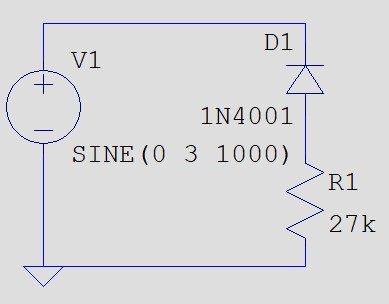
\includegraphics[height=15em]{Images/Circuit2Reverse.jpg}
    \caption{Reverse bias AC circuit}
\end{figure}

The difference between this circuit and the last is the direction
of the diode.

\subsubsection{\(V_\text{out}\) across resistor} This circuit
is again called a series diode clipper like the last one,
but the direction of the diode is switched, and will therefore
clip the positive alternation of \(V_\text{in}\) instead of the
negative alternation. Due to KVL, \(V_\text{out}\) will follow
the following function:
\begin{equation}
    V_\text{out} =
    \begin{cases}
        V_\text{in} + V_f & \text{if $V_\text{in} < -V_f$}\\
        0                 & \text{if $V_\text{in} \ge -V_f$}
    \end{cases}
\end{equation}

This piecewise function is more or less the opposite
of the negative-clipping variant of this circuit. Instead
of cutting off the negative portion of \(V_\text{in}\),
\(V_\text{out}\) is simply \SI{0}{V} during the positive
alternation, and just above \(V_f\) above \(V_\text{in}\)
during the negative alternation. In both cases,
\(|V_\text{in} - V_\text{out}| = V_f\).

\subsubsection{\(V_\text{out}\) across diode} Once again, if
\(V_\text{out}\) is measured across the diode instead of the
resistor, you get a shunt diode clipper; however, instead of
clipping the positive alternation, this circuit clips the
negative alternation. \(V_\text{out}\) will follow the
following function:
\begin{equation}
    V_\text{out} =
    \begin{cases}
        V_\text{in} & \text{if $V_\text{in} > -V_f$}\\
        -V_f         & \text{if $V_\text{in} \le -V_f$}
    \end{cases}
\end{equation}

Again, this function is almost the opposite of its negative-clipping
counterpart. \(V_\text{out}\) follows \(V_\text{in}\) during its
positive alternation, and is capped at \(-V_f\) during its negative
alternation.

\subsubsection{Results} Below is the output of the simulation
of this circuit for both outputs. The sine wave (labeled \texttt{V[n001]} or Trace 3)
represents \(V_\text{in}\). Trace 1, labeled \texttt{V[N001, N002]},
represents the shunt diode clipper; and Trace 2, labeled
\texttt{V[n002]}, is the series diode clipper.

\begin{figure}[h]
    \centering
    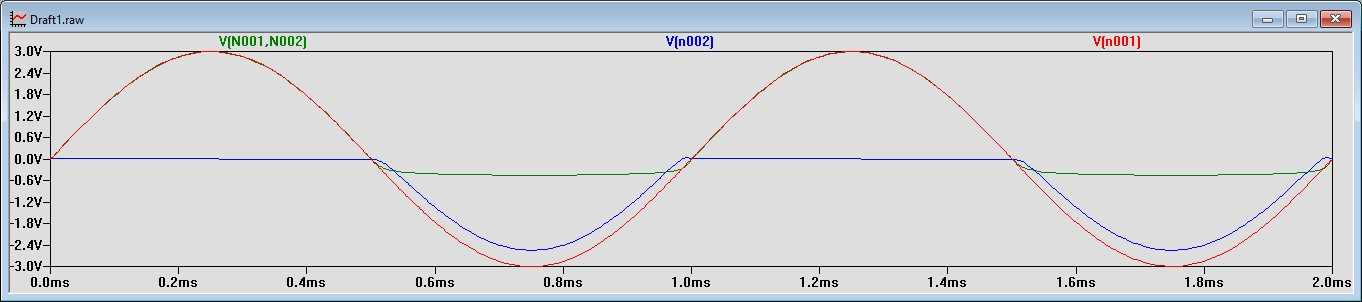
\includegraphics[width=\textwidth]{Images/3VACReverse.jpg}
    \caption{Output for both circuits}
\end{figure}

Both Trace 1 and Trace 2 are merely rigid transformations of their
previous counterparts, being reflected over the time axis and
shifted over one period.
Once again, \(V_\text{in}\) is \(\SI{6}{V}_{pp}\). \(V_{\text{out},R}\)
is \(\SI{2.3}{V}_{pp}\), and \(V_{\text{out},D}\) is \(\SI{3.7}{V}_{pp}\).

\end{document}